% !TEX root = template.tex

\section{Results}
\label{sec:results}

\subsection{\gls{dsrc}}

In the scenario described in \ref{sec:dsrc_model}, Montecarlo simulations have been performed, 15 runs for each distance and for each data rate have been simulated using each time a different random number generator's seed. The results have been elaborated to analyze mean throughput, mean latency, mean \gls{snr} and \gls{ber}.
The outcoming is plotted in \fig{fig:dsrc-throughput}, \fig{fig:dsrc-latency}, \fig{fig:dsrc-SNR} and \fig{fig:dsrc-BER}.

\begin{figure}[ht]
  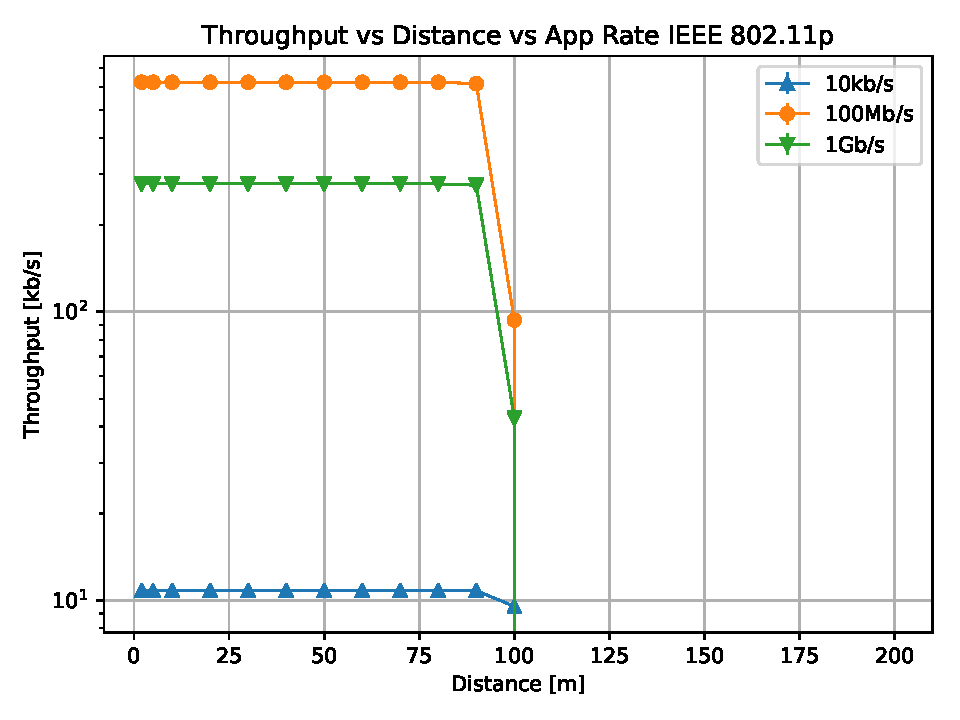
\includegraphics[width=\linewidth]{throughput_distance_wave_UDP}
  \caption{Throughput comparison for 3 different application data rates}
  \label{fig:dsrc-throughput}
\end{figure}

\begin{figure}[ht]
  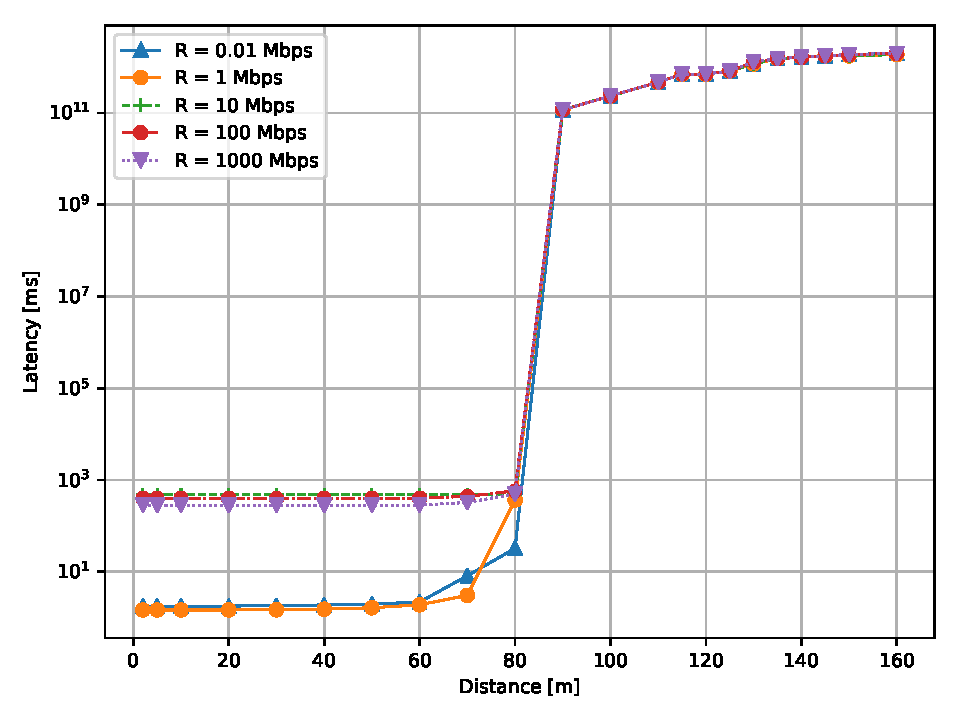
\includegraphics[width=\linewidth]{latency_distance_wave_UDP}
  \caption{Latency comparison for 3 different application data rates}
  \label{fig:dsrc-latency}
\end{figure}

\begin{figure}[ht]
  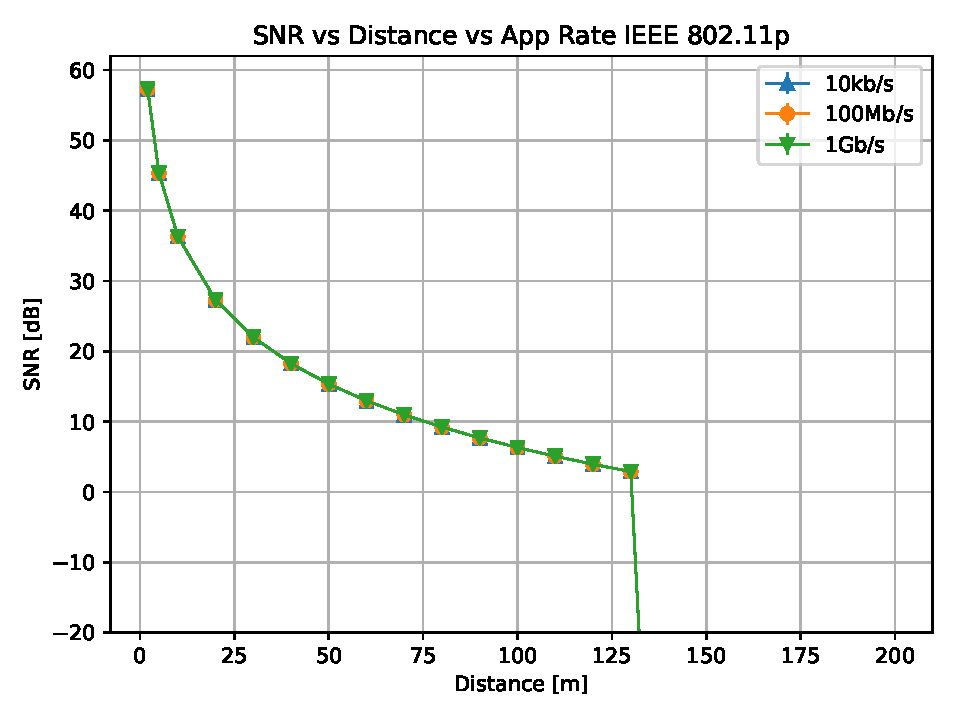
\includegraphics[width=\linewidth]{SNR_distance_wave_UDP}
  \caption{\gls{snr} comparison for 3 different application data rates}
  \label{fig:dsrc-SNR}
\end{figure}

\begin{figure}[ht]
  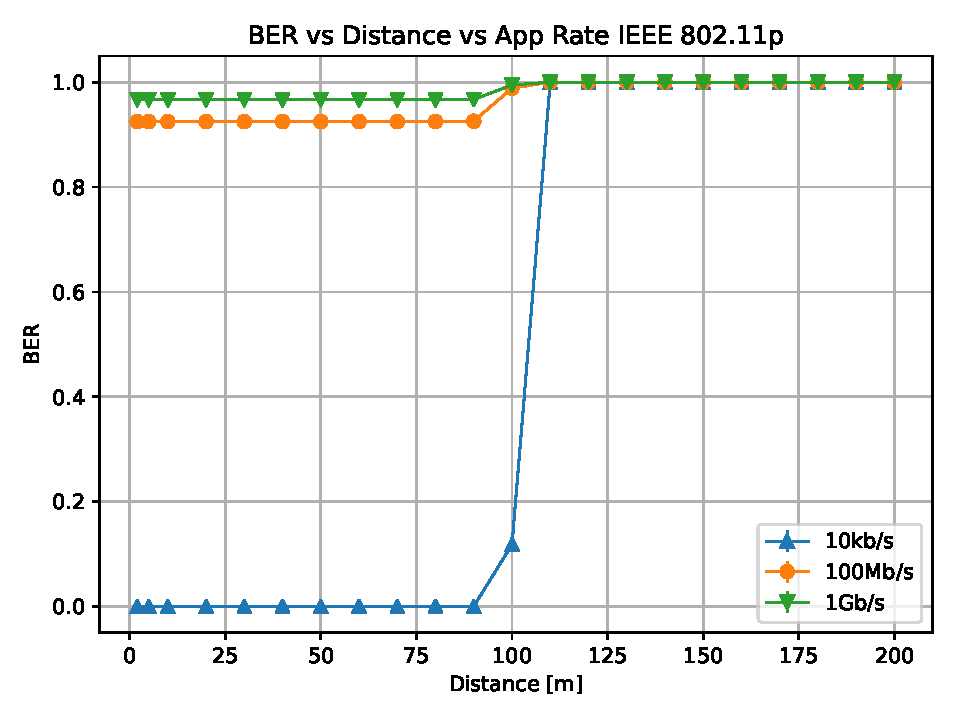
\includegraphics[width=\linewidth]{BER_distance_wave_UDP}
  \caption{\gls{ber} comparison for 3 different application data rates}
  \label{fig:dsrc-BER}
\end{figure}

Looking at the throughput, the only data rate well supported by this technology is the lower one, $10kb/s$, indeed the usual datarates available for \gls{dsrc} are 6, 9, 12, 18, 24, and 27 Mbps with a 10 MHz bandwidth or 6, 9, 12, 18, 24, 36, 48, and 54 Mbps with 20 MHz bandwidth. 
In this simulation a 10 MHz channel has been used with a physical datarate of 6Mbps.
In the case of the lower application datarate, the actual datarate of the communication is slight higher than $10kb/s$, for higher application datarates the physical datarate reached during the transmission is $200kb/s$ for the communication at $1Gb/s$ and $500kb/s$ for the other one, dramatically lower than the application datarate.

Comparing these results with the latency and the \gls{ber}, can be seen as they are approximately 0 for the lower datarate, while for the higher ones, the latency is around 250ms and the \gls{ber} is close to 1. The \gls{ber} for the simulation at $100Mb/s$ is slight lower than the one measured at $1Gb/s$, this implies that the MAC layer of the transmitter has elaborated and sent successfully more packets at the cost of a very high latency. In the higher frequency case, less packets are sent successfully by the transmitter and so the latency measured at the receiver is a bit less.

This is only a matter of representation since the \gls{ber} demonstrates as almost all the packets are lost.

With a distance higher than 100 meters, the \gls{snr} is too low and a communication is impossible, indeed the throughput after 100 meters is 0, the latency and the SNR are not defined and the \gls{ber} is equal to 1.

\subsection{LTE and mmWaves}

Also in this part of the work, Montecarlo simulations has been used with 36 runs for each value of $\lambda_{bs}$ (the base station's density in the simulation area) in the case of \gls{mmWaves} and 18 runs in case of LTE.

The metrics here presented are mean throughput, mean latency, \gls{ber} and \gls{sinr}, plotted respectively in \fig{fig:mmWaves-throughput}, \fig{fig:mmWaves-latency}, \fig{fig:mmWaves-BER} and \fig{fig:mmWaves-SINR}.

\begin{figure}[ht]
  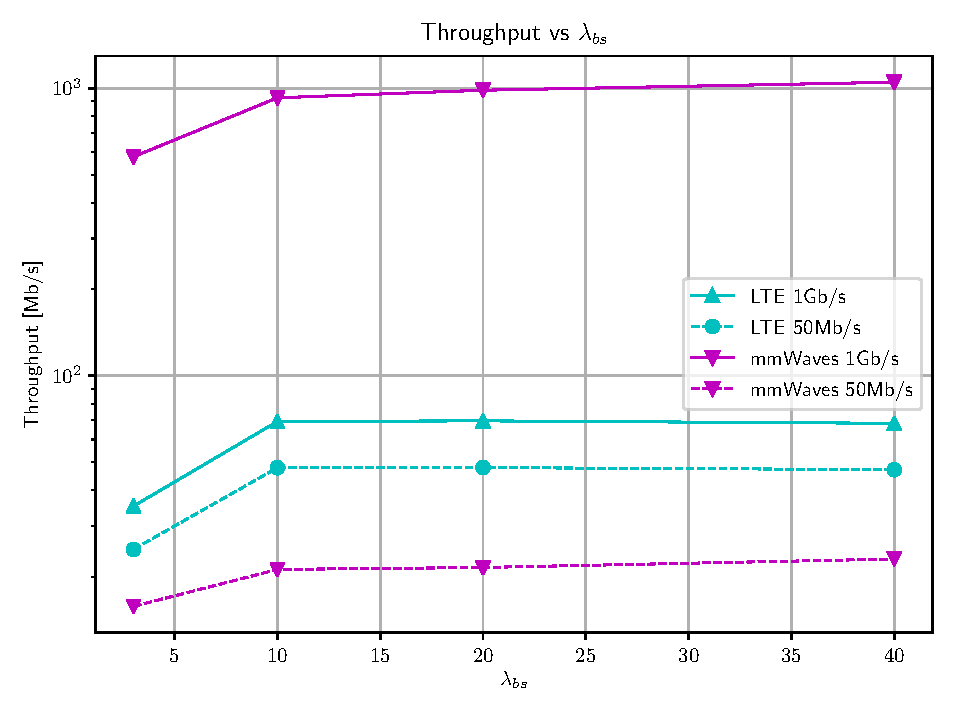
\includegraphics[width=\linewidth]{throughput_lambda_bs_lte_mmwave_UDP}
  \caption{Throughput comparison for LTE and mmWaves}
  \label{fig:mmWaves-throughput}
\end{figure}

\begin{figure}[ht]
  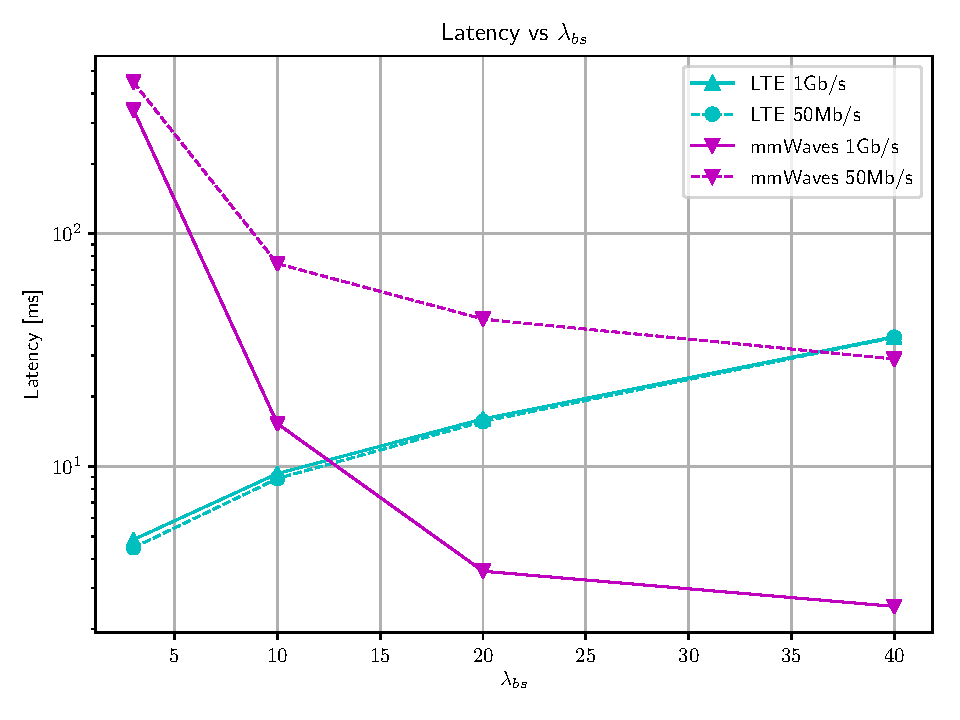
\includegraphics[width=\linewidth]{latency_lambda_bs_lte_mmwave_UDP}
  \caption{Latency comparison for LTE and mmWaves}
  \label{fig:mmWaves-latency}
\end{figure}

\begin{figure}[ht]
  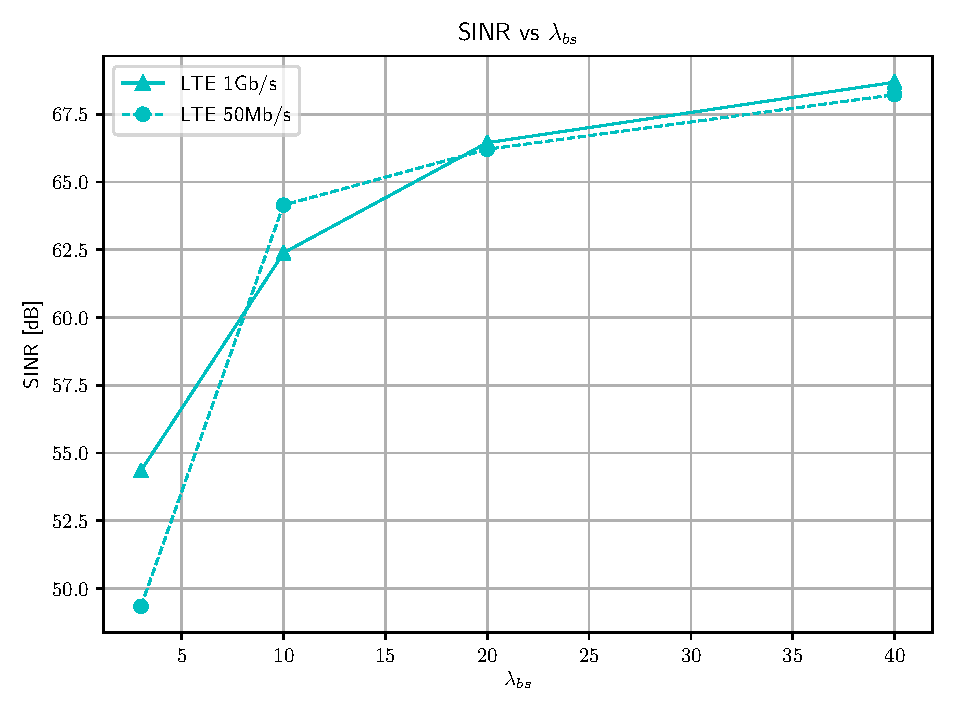
\includegraphics[width=\linewidth]{SINR_lambda_bs_lte_mmwave_UDP}
  \caption{\gls{sinr} comparison for LTE and mmWaves}
  \label{fig:mmWaves-SINR}
\end{figure}

\begin{figure}[ht]
  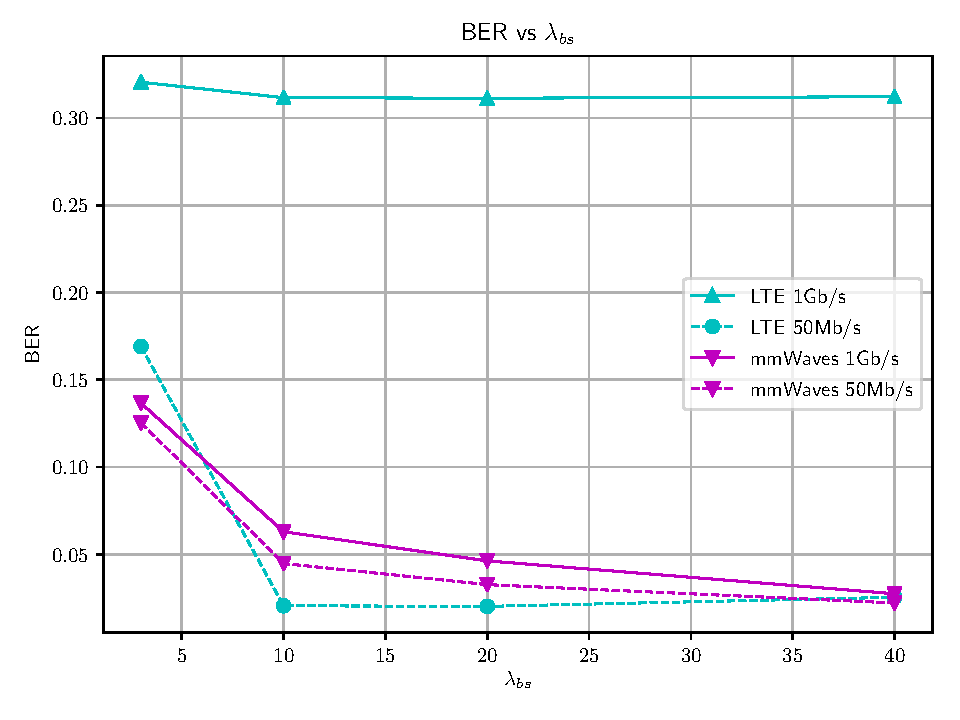
\includegraphics[width=\linewidth]{BER_lambda_bs_lte_mmwave_UDP}
  \caption{\gls{ber} comparison for LTE and mmWaves}
  \label{fig:mmWaves-BER}
\end{figure}

In all the plots, the confidence intervals are missing since more simulations are needed to reduce the variance on data and have statistically robust results. Unfortunately, given the high density of base stations, the simulation time is long and does not allow a large amount of runs.

Even with a reduced number of simulations, can be seen as using \gls{mmWaves}, the throughput is increasing with the number of \gls{gnb}s per $km^2$, while the latency and the \gls{ber} have the opposite behavior.
LTE latency is increasing with the number of \gls{bs} for any datarate used, this is probably due to some imprecision in the code or in the simulator and can be solved in a future work.
It should be noted that latency is computed only on the corrected received packets, so does not take into account the period in which the \gls{ue} is in outage.

In presence of few base stations (in this case 3 base stations is the minimum density simulated), the \gls{ue} can be often in \gls{nlos} because of the distance from the closest base station or the presence of buildings between the \gls{ue} and the \gls{bs}. In these case, mmWave suffers of an high blockage phenomena and, in most cases, it is unable to enstablish a connection in \gls{nlos}, while LTE can still communicate given its lower frequency. As the density increases, \gls{ue} can be often make handover towards a \gls{bs} that ensures a more reliable communication, with a consequent decrease of the mean \gls{ber}.

Looking at the \gls{ber} plot, LTE has high values using 1Gb/s as application datarate, while is lower and it has a decreasing trend for lower datarates. This shows how LTE can not afford such an high datarate.

In the following, an example of a single run for LTE and mmWaves is showed. The user is moving in the same scenario used before with 3 \gls{bs} and 6 buildings.
\fig{fig:mmWaves-throughput-single} and \fig{fig:mmWaves-latency-single} show a mmWave run in which for the first 2.5 seconds the \gls{ue} is in \gls{nlos}, from 2.5 to 4.5 seconds \gls{ue} is in \gls{los} and receives all the packets while for the remaining time it is in outage and no packets are received.
In the LTE run, \fig{fig:lte-throughput-single} and \fig{fig:lte-latency-single} show that throughput and latency are almost constant despite the buildings, since LTE uses a lower frequency. They have an abnormal behavior after 4 seconds since the \gls{ue} is moving and it goes in \gls{nlos}. From 5 to 10 seconds the \gls{ue} is in outage and no measures are taken.

\begin{figure}[ht]
  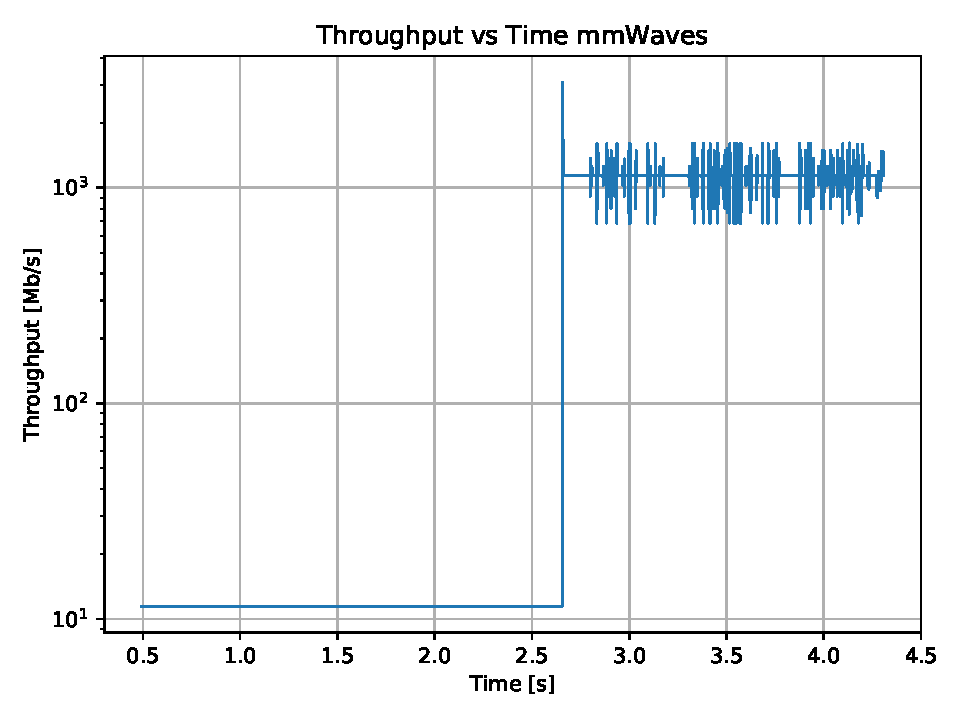
\includegraphics[width=\linewidth]{throughput_mmWaves_UDP}
  \caption{Throughput registered in a single run using mmWaves}
  \label{fig:mmWaves-throughput-single}
\end{figure}

\begin{figure}[ht]
  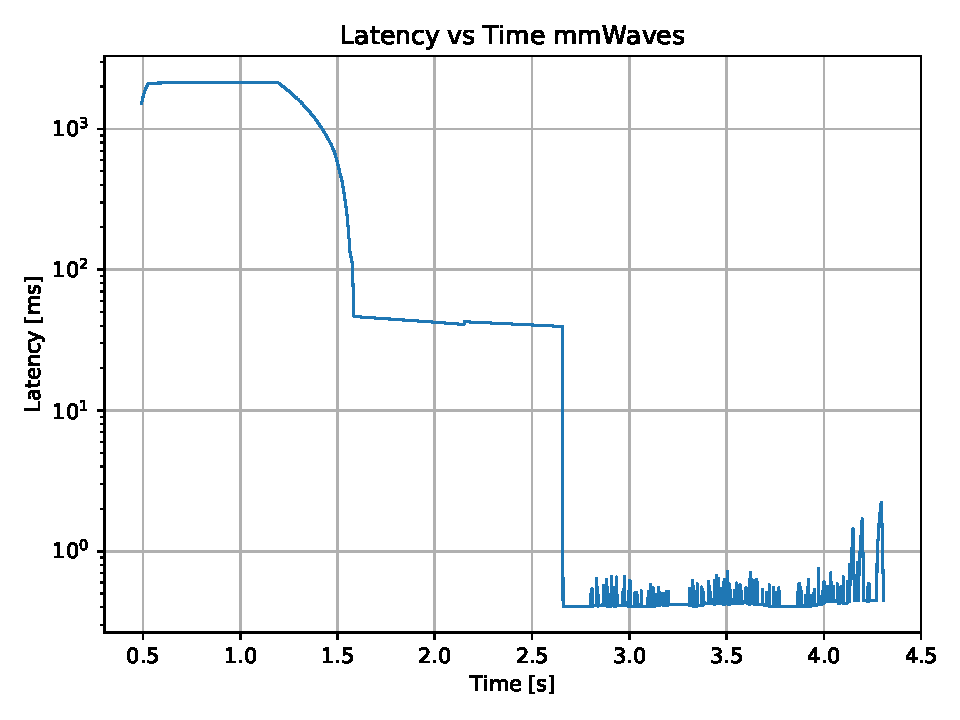
\includegraphics[width=\linewidth]{latency_mmWaves_UDP}
  \caption{Latency registered in a single run using mmWaves}
  \label{fig:mmWaves-latency-single}
\end{figure}

\begin{figure}[ht]
  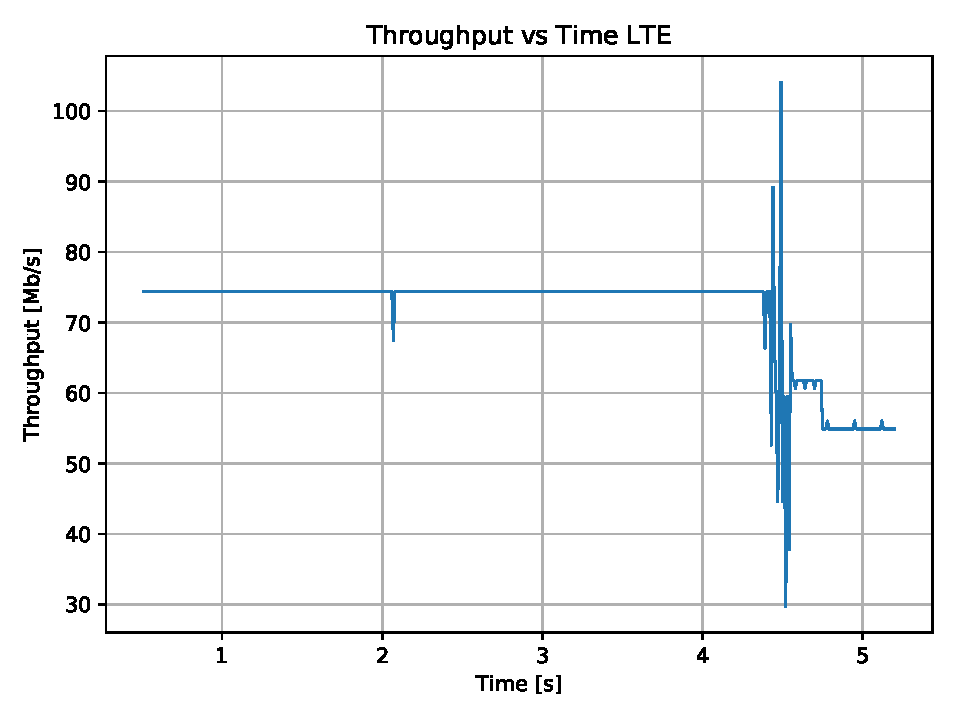
\includegraphics[width=\linewidth]{throughput_lte_UDP}
  \caption{Throughput registered in a single run using LTE}
  \label{fig:lte-throughput-single}
\end{figure}

\begin{figure}[ht]
  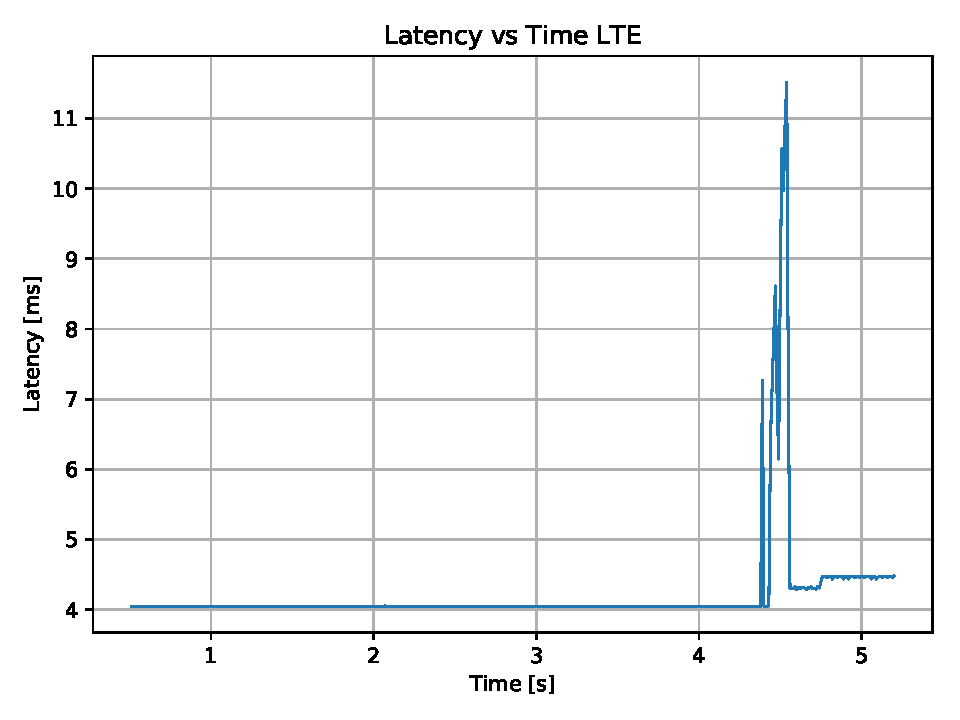
\includegraphics[width=\linewidth]{latency_lte_UDP}
  \caption{Latency registered in a single run using LTE}
  \label{fig:lte-latency-single}
\end{figure}